\chapter{Analytic Solutions to the Neutron Diffusion Equation}
\label{ap:analyticSolutions}

\section{Introduction}
  The following are analytic solutions designed for verification of one-,
  two-, and three-dimension numerical neutron diffusion equation solvers.
  One-group and two-group problems are also addressed.
  
  For the reference problems, the one-group neutron diffusion problem is written
  below.
  \begin{equation} \label{eq:onegroup}
    -D \grad^2 \phi + \Sigma_r \phi =  \frac{1}{\keff} \nu \Sigma_f \phi + 
      q_{fixed}
  \end{equation}
  Where $\grad^2 \phi = \grad \cdot (\grad \phi)$ and is used to simplify 
  notation. For two-group neutron diffusion problems, the two-group neutron 
  diffusion problem is written below.
  \begin{align} 
    \label{eq:twogroup1}
    -D_1 \grad^2 \phi_1 + \Sigma_{r1} \phi_1 &= \frac{1}{\keff} \left(
      \nu \Sigma_{f1} \phi_1 + \nu \Sigma_{f2} \phi_2 \right) \\
    \label{eq:twogroup2}
    -D_2 \grad^2 \phi_2 + \Sigma_{r2} \phi_2 &= 
      \Sigma_{s 1 \rightarrow 2} \phi_2
  \end{align}
  Where $\phi_1$ is the higher energy group and $\phi_2$ is the lower energy 
  group. This formulation assumes all fission neutrons are created in the fast 
  energy group and there is no up-scattering (scattering that results in an 
  increase in neutron energy). These are realistic assumptions for all diffusive
  neutron systems.

  Analytic solutions are provided herein. One-dimension problems can be 
  replicated in a two-dimension solver using a square geometry and select 
  boundary conditions. For a given quadrilateral, two of the boundary conditions
  are set to reflective conditions and two are set to zero-flux $(\phi = 0)$ 
  conditions. For true two-dimensions problems, all of the boundary conditions 
  are set to zero-flux conditions.
  
  These formula are common to second order partial differential equations but
  the formulation here is based in part from \cite{textbooklewis}.

\section{One-Dimension, One-Group, Fixed Source}
  \label{sec:deriv_1dfixedsrc}
  This one-dimension problem is in the domain $x \in [0,L_x]$. The material is
  homogeneous within the problem and has fixed coefficient properties.
  The problem is specified in \eref{eq:1dfixed}, \eref{eq:1dfixed_bc1}, and 
  \eref{eq:1dfixed_bc2}.
  \begin{equation}
    \label{eq:1dfixed}
    -D \frac{d^2}{dx^2} \phi(x) + \Sigma_r \phi(x) = q_{fixed}
  \end{equation}
  \begin{align}
    \label{eq:1dfixed_bc1}
    \phi(0) &= 0 \\
    \label{eq:1dfixed_bc2}
    \phi(L_x) &= 0
  \end{align}
  \eref{eq:1dfixed} can be rewritten as
  \begin{equation}
    \label{eq:1dfixed_buckle}
    \frac{d^2}{dx^2} \phi(x) - B^2 \phi(x) = q_{fixed}
  \end{equation}
  Where $B$ is the buckling term and is given for this problem in
  \eref{eq:1dfixed_b2}.
  \begin{equation}
    \label{eq:1dfixed_b2}
    B^2 = \frac{\Sigma_r}{D}
  \end{equation}
  Begin the solution by allowing to be composed of homogeneous and particular
  solutions. 
  \begin{equation} 
    \phi(x) = \phi_h(x) + \phi_p(x)
  \end{equation}
  Using the form of \eref{eq:1dfixed_buckle}, the homogeneous solution satisfies 
  equation \eref{eq:1dfixed_homog}.
  \begin{equation}
    \label{eq:1dfixed_homog}
    \frac{d^2}{dx^2} \phi_x(x) - B^2 \phi_h(x) = 0
  \end{equation}
  The homogeneous solution $\phi_h(x)$ has form \eref{eq:1dfixed_homog_form}.
  \begin{equation}
    \label{eq:1dfixed_homog_form}
    \phi_h(x) = c_1 \, \cosh(B \, x) + c_2 \, \sinh(B \, x)
  \end{equation}
  The particular solution is given for a constant value $q_{fixed}$ in
  \eref{eq:1dfixed_particular}.
  \begin{equation}
    \label{eq:1dfixed_particular}
    \phi_p(x) = -\frac{q_{fixed}}{B^2}
  \end{equation}
  Where $B^2$ comes from \eref{eq:1dfixed_b2}. Combining homogeneous and 
  particular solutions.
  \begin{equation}
    \label{eq:1dfixed_constants}
    \phi(x) = c_1 \, \cosh(B \, x) + c_2 \, \sinh(B \, x) -
      \frac{q_{fixed}}{B^2}
  \end{equation}
  Next, boundary conditions are considered with \eref{eq:1dfixed_constants}.
  Beginning with the boundary at $x=0$ as specified in \eref{eq:1dfixed_bc1}.
  \begin{align}
    \phi(0) &= 0 \\
    &= c_1 - \frac{q_{fixed}}{B^2} \\
    \label{eq:1dfixed_c1}
    c_1 &= \frac{q_{fixed}}{B^2}
  \end{align}
  \eref{eq:1dfixed_c1} is then inserted into \eref{eq:1dfixed_constants}.
  \begin{align}
    \phi(x) &= \frac{q_{fixed}}{B^2} \, \cosh(B\, x) + c_2 \,
      \sinh(B \, x) - \frac{q_{fixed}}{B^2} \\
    \phi(x) &= \frac{q_{fixed}}{B^2} \left( \cosh(B\, x) -1 \right)
      + c_2 \, \sinh(B \, x)
  \end{align}
  The next boundary condition is evaluated at $x=L_x$ as apecified in
  \eref{eq:1dfixed_bc2}.
  \begin{align}
    \phi(L_x) &= 0 \\
    &= \frac{q_{fixed}}{B^2} \left( \cosh(B \, L_x ) - 1 \right) + c_2 \,
      \sinh(B \, L_x) \\
    \label{eq:1dfixed_c2}
    c_2 &= \frac{\frac{q_{fixed}}{B^2} \left(\cosh(B \, L_x) -1 \right)}
      {\sinh(B \, L_x)}
  \end{align}
  All constants of the problem are now specified in \eref{eq:1dfixed_c1} and 
  \eref{eq:1dfixed_c2} and can be substitued into \eref{eq:1dfixed_constants}.
  \begin{equation}
    \label{eq:analytic_1dfixedsrc}
    \phi(x) = \frac{q_{fixed}}{B^2} \left( \cosh(B\,x)-1 \right) +
    \frac{\frac{q_{fixed}}{B^2} \left(\cosh(B\,L_x)-1\right)}{\sinh(B\,L_x)}
    \sinh(B\,x)
  \end{equation}
  The result in \eref{eq:analytic_1dfixedsrc} is presented in
  \fref{fig:fixed_critical}. Note that the magnitude of the function is not
  arbitrary and is specified by the coefficients of the problem.
  \begin{figure}
    \centering
    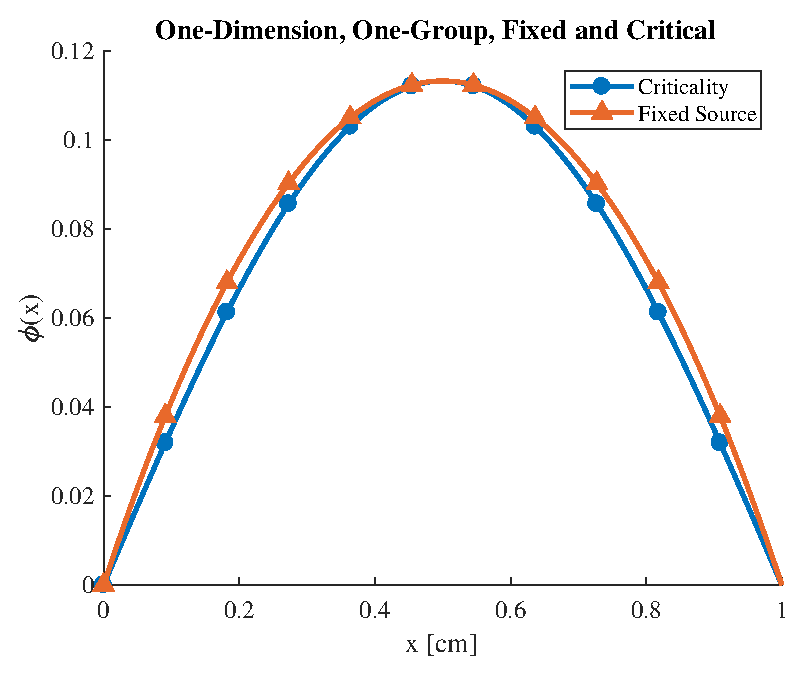
\includegraphics[width=0.7\textwidth]{fixed_critical}
    \caption{Fixed Source and Criticality Flux Shapes for One-Dimension,
      One-Group Problems.}
    \label{fig:fixed_critical}
  \end{figure}
  
\section{One-Dimension, One-Group, Criticality} 
  \label{sec:deriv_1d1g}
  This one-dimension problem is in the domain $x \in [0,L_x]$. The material
  is homogeneous within the problem and has fixed coefficient properties. The
  problem is specified in \eref{eq:1d1g}, \eref{eq:1d1g_bc1}, and
  \eref{eq:1d1g_bc2}.
  \begin{equation}
    \label{eq:1d1g}
    -D \frac{d^2}{dx^2} \phi(x) + \Sigma_r \phi(x) = 
      \frac{1}{\keff} \nu \Sigma_f \phi(x)
  \end{equation}
  \begin{align}
    \label{eq:1d1g_bc1}
    \phi(0) &= 0 \\
    \label{eq:1d1g_bc2}
    \phi(L_x) &= 0
  \end{align}
  \eref{eq:1d1g} can be rewritten as
  \begin{equation}
    \label{eq:1d1g_buckle}
    \frac{d^2}{dx^2} \phi(x) + B^2 \phi(x) = 0
  \end{equation}
  Where $B$ is the buckling term and is given for this problem in
  \eref{eq:1d1g_b2}.
  \begin{equation}
    \label{eq:1d1g_b2}
    B^2 = \frac{\frac{1}{\keff} \nu \Sigma_f - \Sigma_r}{D}
  \end{equation}
  \eref{eq:1d1g_buckle} has general solution given in \eref{eq:1d1g_general}.
  \begin{equation}
    \label{eq:1d1g_general}
    \phi(x) = c_1 \, \cos(B \, x) + c_s \, \sin(B \, x)
  \end{equation}
  Using \eref{eq:1d1g_general}, the boundary condition is applied at $x=0$ as
  specified in \eref{eq:1d1g_bc1}.
  \begin{align}
    \phi(0) &= 0 \\
    &= c_1 \\
    \label{eq:1d1g_c1}
    c_1 &= 0
  \end{align}
  \eref{eq:1d1g_c1} is then inserted into \eref{eq:1d1g_general}.
  \begin{equation}
    \label{eq:1d1g_sin}
    \phi(x) = c_2 \, \sin(B \, x)
  \end{equation}
  Next, the boundary condition is evaluated at $x=L_x$ as specified in
  \eref{eq:1d1g_bc2}.
  \begin{align}
    \phi(L_x) &= 0 \\
    &= c_2 \, \sin(B \, L_x)
  \end{align}
  For a non-trivial solution, this problem is an eigenvalue problem with $B$
  specified by the boundary condition. This implies $c_2$ is arbitrary and the
  magnitude of the flux can be normalized to a constant. For simplicity, allow
  $c_2 = 1$. Then, recall the zeros of the sine function.
  \begin{align}
    B \, L_x &= n \, \pi \\
    B &= \frac{n \, \pi}{L_x}
  \end{align}
  Where $n$ is an integer. For the fundamental mode, $n=1$.
  \begin{equation}
    \label{eq:1d1g_buckle_geom}
    B = \frac{\pi}{L_x}
  \end{equation}
  Substitute \eref{eq:1d1g_buckle_geom} into \eref{eq:1d1g_sin} for the final
  solution to the fundamental eigenmode.
  \begin{equation}
    \label{eq:analytic_1d1g}
    \phi(x) = \sin\left(\frac{\pi}{L_x} x \right)
  \end{equation}
  This flux shape is plotted in \fref{fig:fixed_critical}. Recall that the
  magnitude is arbitrary so the flux is normalized to have maximum equal to the
  fixed solution for visualization purposes.
  Recalling the definition of $B$ from \eref{eq:1d1g_b2}, the fundamental
  eigenvalue of the problem, $\keff$, can be solved.
  \begin{align}
    \frac{\pi}{L_x} &= 
      \sqrt{\frac{\frac{1}{\keff} \nu \Sigma_f - \Sigma_r}{D}} \\
    \label{eq:keff1d}
    \keff &= \frac{\nu \Sigma_f}{D \left(\frac{\pi}{L_x}\right)^2 + \Sigma_r}
  \end{align}
  Using material properties given in \tref{tab:1group_simple} and $L_x =
  \units{cm}$, then
  \begin{equation}
    \keff = 1.998028
  \end{equation}

  \begin{table}
    \caption{One-Group Sample Cross Sections.}
    \label{tab:1group_simple}
    \begin{center}
      \begin{tabular}{cc}
        \toprule
        Cross Section & Value \\
        \midrule
        $D \units{$\frac{1}{\text{cm}}$} $ & 1 \\
        $\Sigma_r \units{cm}$& 1 \\
        $ \nu \Sigma_{f} \units{cm} $ & 2 \\
        \bottomrule
      \end{tabular}
    \end{center}
  \end{table}

\section{Two-Dimension, One-Group, Criticality}
  \label{sec:deriv_2d1g}
  This two-dimension problem is in the rectangular domain $[0,L_x] \times
  [0,L_y]$. That is, $x \in [0,L_x]$ and $y \in [0,L_y]$. The material is
  homogeneous within the problem and has fixed coefficient properties. The
  problem is specified in \eref{eq:2d1g}, \eref{eq:2d1g_bc1},
  \eref{eq:2d1g_bc2}, \eref{eq:2d1g_bc3}, and \eref{eq:2d1g_bc4}.
  \begin{equation}
    \label{eq:2d1g}
    -D \grad^2 \phi(x,y) + \Sigma_r \phi(x,y) = 
      \frac{1}{\keff} \nu \Sigma_f \phi(x,y)
  \end{equation}
  \begin{align}
    \label{eq:2d1g_bc1}
    \phi(0,y) &= 0 \\
    \label{eq:2d1g_bc2}
    \phi(L_x,y) &= 0 \\
    \label{eq:2d1g_bc3}
    \phi(x,0) &= 0 \\
    \label{eq:2d1g_bc4}
    \phi(x,L_y) &= 0
  \end{align}
  Noting in \eref{eq:2d1g} that $\grad^2 \phi = \grad \cdot (\grad \phi)$.
  \eref{eq:2d1g} can be rewritten as
  \begin{equation}
    \label{eq:2d1g_buckle}
    \grad^2 \phi(x,y) + B^2 \phi(x,y) = 0
  \end{equation}
  Where $B$ is the buckling term and is given for this problem in
  \eref{eq:2d1g_b2}.
  \begin{equation}
    \label{eq:2d1g_b2}
    B^2 = \frac{\frac{1}{\keff} \nu \Sigma_f - \Sigma_r}{D}
  \end{equation}
  The Laplacian $\grad^2$ in \eref{eq:2d1g_buckle} is then expanded into partial
  derivatives.
  \begin{equation}
    \label{eq:2d1g_partial}
    \frac{\partial^2}{\partial x^2} \phi(x,y) + \frac{\partial^2}{\partial y^2}
      \phi(x,y) + B^2 \phi(x,y) = 0
  \end{equation}
  The method of separation of variables will be used to solve
  \eref{eq:2d1g_partial}. Begin by assuming that $\phi(x,y)$ is separable as in
  \eref{eq:2d1g_separable}.
  \begin{equation}
    \label{eq:2d1g_separable}
    \phi(x,y) = X(x)\,Y(y)
  \end{equation}
  Then, inserting \eref{eq:2d1g_separable} into \eref{eq:2d1g_partial}.
  \begin{align}
    \frac{\partial^2}{\partial x^2} \left( X(x)\,Y(y) \right) + 
      \frac{\partial^2}{\partial y^2} \left( X(x)\,Y(y) \right) + 
      B^2 X(x)\,Y(y) &= 0 \\
    \label{eq:2d1g_above}
    Y(y) \frac{\partial^2}{\partial x^2} X(x) + 
      X(y) \frac{\partial^2}{\partial y^2} Y(x) + 
      B^2 X(x) \, Y(y) &= 0
  \end{align}
  Divide \eref{eq:2d1g_above} by the quantity $X(x)\,Y(y)$.
  \begin{equation}
    \label{eq:2d1g_divide_sum}
    \frac{1}{X(x)} \, \frac{d^2}{d x^2} X(x) + 
      \frac{1}{Y(y)} \, \frac{d^2}{d y^2} Y(y) + 
      B^2 = 0
  \end{equation}
  Each of the partial derivatives operates on a function of only one variable so
  the derivatives become standard derivatives.

  The first two terms of \eref{eq:2d1g_divide_sum} are function of only $x$ and
  $y$ respectively, and their sum is equal to a constant. Therefore, both of the
  terms must also be equal to a constant \cite{lamarsh1966}. Splitting
  \eref{eq:2d1g_divide_sum} into two equations yields
  \begin{align}
    \label{eq:2d1g_x}
    \frac{1}{X(x)} \, \frac{d^2}{d x^2} X(x) + \alpha^2 &= 0 \\
    \label{eq:2d1g_y}
    \frac{1}{Y(y)} \, \frac{d^2}{d y^2} Y(y) + \beta^2 &= 0
  \end{align}
  where $\alpha$ and $\beta$ are constants such that
  \begin{equation}
    \label{eq:2d1g_buckle_alphabeta}
    \alpha^2 + \beta^2 = B^2
  \end{equation}
  Consider \eref{eq:2d1g_x} and boundary conditions specified in
  \eref{eq:2d1g_bc1} and \eref{eq:2d1g_bc2}. Then, \eref{eq:2d1g_x} can be
  rewritten
  \begin{equation}
    \frac{d^2}{dx^2} X(x) + \alpha^2 X(x) = 0
  \end{equation}
  this is similar to the previous problem in \eref{eq:1d1g_buckle} which has 
  general solution of the form
  \begin{equation}
    \label{eq:2d1g_x_general}
    X(x) = c_1 \, \cos(\alpha \, x) + c_2 \, \sin(\alpha \, x)
  \end{equation}
  Consider the boundary condition at $x=0$ as specified in \eref{eq:2d1g_bc1}.
  \begin{align}
    X(0) &= 0 \\
    &= c_1 \\
    \label{eq:2d1g_x_c1}
    c_1 &= 0
  \end{align}
  Inserting the result \eref{eq:2d1g_x_c1} into \eref{eq:2d1g_x_general}.
  \begin{equation}
    \label{eq:2d1g_x_sin}
    X(x) = c_2 \, \sin( \alpha x)
  \end{equation}
  Then considering the boundary condition at $x=L_x$ as specified in
  \eref{eq:2d1g_bc2}.
  \begin{align}
    X(L_x) &= 0 \\
    &= c_2 \, \sin(\alpha \, L_x)
  \end{align}
  For non-trivial solution $X(x)$, this is an eigenvalue problem with $\alpha$
  specified by the boundary condition. This implies $c_2$ is arbitrary and the
  magnitude of the function can be normalized to a constant. For simplicity,
  allow $c_2 = 1$. Then, recall the zeros of the sine function.
  \begin{align}
    \alpha \, L_x &= n \, \pi \\
    \alpha &= \frac{n \, \pi}{L_x}
  \end{align}
  Where $n$ is an integer. For the fundamental mode $n=1$.
  \begin{align}
    \label{eq:2d1g_x_alpha}
    \alpha = \frac{\pi}{L_x}
  \end{align}
  Substitute \eref{eq:2d1g_x_alpha} into \eref{eq:2d1g_x_sin} for the solution
  to the fundamental mode of $X(x)$.
  \begin{equation}
    \label{eq:2d1g_x_solution}
    X(x) = \sin\left(\frac{\pi}{L_x} x \right)
  \end{equation}
  Similar procedure is performed to solve for $Y(y)$.
  \begin{equation}
    \label{eq:2d1g_y_solution}
    Y(y) = \sin\left(\frac{\pi}{L_y} y \right)
  \end{equation}
  \eref{eq:2d1g_x_solution} and \eref{eq:2d1g_y_solution} are substituted into
  \eref{eq:2d1g_separable}.
  \begin{equation}
    \label{eq:analytic_2d1g}
    \phi(x,y) = \sin\left(\frac{\pi}{L_x} x\right) \, 
      \sin\left(\frac{\pi}{L_y} y\right)
  \end{equation}
  The flux shape in \eref{eq:analytic_2d1g} is plotted in \fref{fig:2d1g}.
  \begin{figure}
    \centering
    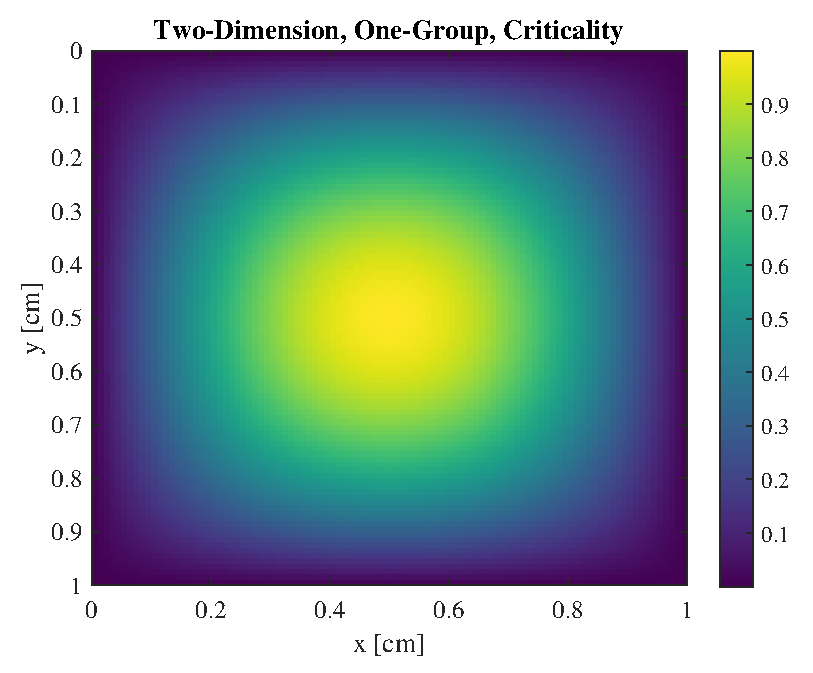
\includegraphics[width=0.7\textwidth]{2d1g}
    \caption{Two-Dimension Criticality Flux Shape.}
    \label{fig:2d1g}
  \end{figure}
  Using \eref{eq:2d1g_buckle_alphabeta} along with \eref{eq:2d1g_x_alpha} and a
  similar expression for $\beta$, the buckling can be written geometrically.
  \begin{equation}
    \label{eq:2d1g_buckle_geom}
    B^2 = \left(\frac{\pi}{L_x}\right)^2 + \left(\frac{pi}{L_y}\right)^2
  \end{equation}.
  Setting \eref{eq:2d1g_buckle_geom} equal to \eref{eq:2d1g_b2} yields an
  expression for $\keff$.
  \begin{align}
    \left(\frac{\pi}{L_x}\right)^2 + \left(\frac{pi}{L_y}\right)^2 &=
      \frac{\frac{1}{\keff} \nu \Sigma_f - \Sigma_r}{D} \\
    \keff &= \frac{\nu \Sigma_f}{D \left( \left(\frac{\pi}{L_x}\right)^2 + 
      \left( \frac{\pi}{L_y}\right)^2 \right) + \Sigma_r}
  \end{align}
  For material coefficients specified in \tref{tab:1group_simple} and
  $L_x=L_y=100 \units{cm}$, 
  \begin{equation}
    \label{eq:keff2d}
    \keff = 1.996060
  \end{equation}
  
\section{One-Dimension, Two-Group, Criticality}
  \label{sec:deriv_1d2g}
  Much of this section is drawn from course notes prepared by Dr. Scott 
  Palmtag \cite{analytic2g}.
  
  A two-group neutron diffusion problem is considered for a one-dimension
  homogeneous slab in the domain $x \in [0,L]$. Energy group 1 is higher energy
  than energy group 2. It is assumed all fission neutrons are  produced in the
  fast group (i.e. $\chi_1=1$ and $\chi_2=0$). Additionally, it is assumed that 
  there is no up-scattering  (i.e. $\Sigma_{2\rightarrow1}=0$).  Then, the
  two-group neutron diffusion equations are given in \eref{eq:twogroup1} and 
  \eref{eq:twogroup2}.
  
  Referring to the problem posed by Section \sref{sec:deriv_1d1g}, the flux 
  solutions have form given in equation \eref{eq:1d1g_sin}. Then
  \begin{align}
    \label{eq:twogroupflux1}
    \phi_1(x) &= c_1 \sin(Bx) \\
    \label{eq:twogroupflux2}
    \phi_2(x) &= c_2 \sin(Bx)
  \end{align}
  Where $B$ is the geometric buckling term. For this geometry, the geometric 
  buckling of the fundamental mode is given by 
  \begin{equation}
    B = \pi/L_x
  \end{equation}
  Then, inserting \eref{eq:twogroupflux1} and \eref{eq:twogroupflux2} into 
  \eref{eq:twogroup2} and dividing the equation by $\sin(Bx)$
  \begin{equation}
    D_2 B^2 c_2 + \Sigma_{r2} c_2 = \Sigma_{s1\rightarrow2} c_1
  \end{equation}
  Then, the ratio can be expressed
  \begin{equation} \label{eq:fluxratio}
    \frac{c_2}{c_1} = \frac{\Sigma_{s1\rightarrow2}}{D_2 B^2 + \Sigma_{r2}}
  \end{equation}
  The ratio $\frac{c_2}{c_1}$ represents the relative magnitude of thermal to 
  fast flux. Returning to \eref{eq:twogroup1}, and using in 
  \eref{eq:twogroupflux1} and \eref{eq:twogroupflux2} and again dividing both
  sides by  $\sin(Bx)$
  \begin{align}
    D_1 B^2 c_1 &= \frac{1}{\keff} \left( \nu \Sigma_{f1} c_1 + 
      \nu \Sigma_{f2} c_2\right)\\
    \keff &= \frac{\nu \Sigma_{f1} c_1 + \nu \Sigma_{f2} c_2}
      {D_1 B^2 c_1 + \Sigma{r1} c_1}\\
    \keff &= \frac{\nu \Sigma_{f1} + \nu \Sigma_{f2} c_2/c_1}
      {D_1 B^2 + \Sigma{r1}}
  \end{align}
  Inserting the expression from \eref{eq:fluxratio}
  \begin{equation}
    \keff = \frac{\nu \Sigma_{f1} + \nu \Sigma_{f2} 
      \left(\frac{\Sigma_{s1\rightarrow2}}{D_2B^2+\Sigma_{r2}}\right)}
      {D_1 B^2 + \Sigma{r1}}
  \end{equation}
  From the VVER-440 benchmark \sref{sec:vver440}, material 1,
  \begin{align*}
    D_1 &= 1.3466  \\
    D_2 &= 0.37169 \\
    \Sigma_{r1} &= 2.5255\text{E}-2\\
    \Sigma_{r2} &= 6.4277\text{E}-2\\
    \nu \Sigma_{f1}  &= 4.4488\text{E}-3\\
    \nu \Sigma_{f2}  &= 7.3753\text{E}-2\\
    \Sigma_{s1\rightarrow2} &= 1.6893\text{E}-2 \\
    k_{\infty} &= 0.943664259
  \end{align*}
  For a 100 \units{cm} slab.
  \begin{align}
    \frac{c_2}{c_1} &= 0.26132419 \\
    \keff &= 0.892349025
  \end{align}
  
\section{One-Dimension, One-Group, Two Region, Criticality}
  \label{sec:deriv_2reg}
  This one-dimension problem is meant to simulate a reactor with reflective
  material at the edge of the reactor. This has the benefit of testing the
  materials mapping of the solver. The problem is in the domain $x \in [0,L_R]$. 
  Geometry is described in \fref{fig:2reg_geom}. Fuel material (subscript F) is
  located in $x \in [0,L_F]$ and reflector material (subscript R) is located in 
  $ x \in [L_F,L_R]$. The material is homogeneous within each respective section
  and has fixed coefficient properties in their region. The problem is specified
  in \eref{eq:2regF}, \eref{eq:2regR}, \eref{eq:2reg_bc0},
  \eref{eq:2reg_flux_continuity}, \eref{eq:2reg_current_continuity},
  \eref{eq:2reg_bcLR}.
  \begin{figure}
    \centering
    \includegraphics[width=0.5\textwidth]{2reg_geom}
    \caption{Geometry for Two Region Problem.}
    \label{fig:2reg_geom}
  \end{figure}
  \begin{align}
    \label{eq:2regF}
    -D_F \frac{d^2}{dx^2} \phi_F(x) + \Sigma_{rF} &= \frac{1}{\keff} \nu
      \Sigma_{fF} \phi_F(x) \qquad \forall \; x \in [0,L_F] \\
    \label{eq:2regR}
    -D_R \frac{d^2}{dx^2} \phi_R(x) + \Sigma_{rR} &= 0 \qquad \forall 
      \; x \in [L_F,L_R]
  \end{align}
  \begin{align}
    \label{eq:2reg_bc0}
    \left. \frac{d}{dx} \phi_F(x) \right|_{x=0} &= 0 \\
    \label{eq:2reg_flux_continuity}
    \phi_F(L_F) &= \phi_R(L_F) \\
    \label{eq:2reg_current_continuity}
    D_F \left. \frac{d}{dx} \phi_F(x) \right|{x=L_F} &= 
      D_R \left. \frac{d}{dx} \phi_R(x) \right|{x=L_F} \\
    \label{eq:2reg_bcLR}
    \phi_R(L_R) &= 0
  \end{align}
  Beginning in the fueled region. The diffusion equation \eref{eq:2regF} can be
  rewritten with a buckling term $B_F$.
  \begin{equation}
    \label{eq:2regF_buckle}
    \frac{d^2}{dx^2} \phi_F(x) + B_F^2 \phi_F(x) = 0 
  \end{equation}
  Where $B_F^2$ is given in \eref{eq:2regF_b2}.
  \begin{equation}
    \label{eq:2regF_b2}
    B_F^2 = \frac{\frac{1}{\keff} \nu \Sigma_{fF} - \Sigma_{rF}}{D_F}
  \end{equation}
  \eref{eq:2regF_buckle} has general solution of the form
  \begin{equation}
    \label{eq:2regF_general}
    \phi_F(x) = c_{1F} \, \cos(B_F\,x) + c_{2F} \, \sin(B_F\,x)
  \end{equation}
  The derivative of \eref{eq:2regF_general} is also provided as it will be
  useful for evaluating boundary conditions.
  \begin{equation}
    \label{eq:2regF_general_derivative}
    \frac{d}{dx}\phi_F(x) = -c_{1F} \, B_F \, \sin(B_F\,x) + 
      c_{2F} \, B_F \, \cos(B_F\,x)
  \end{equation}
  Using \eref{eq:2regF_general_derivative}, the boundary condition is evaluated
  at $x=0$ as specified in \eref{eq:2reg_bc0}.
  \begin{align}
    \phi_F(0) &= 0 \\
    &= c_{2F} \, B_F \\
    \label{eq:2reg_c2f}
    c_{2F} &= 0
  \end{align}
  \eref{eq:2reg_c2f} is inserted into \eref{eq:2regF_general}
  \begin{equation}
    \label{eq:2regF_cos}
    \phi_F(x) = c_{1F} \, \cos(B_F\, x)
  \end{equation}
  and its derivative is provided.
  \begin{equation}
    \label{eq:2regF_cos_derivative}
    \frac{d}{dx} \phi_F(x) = -c_{1F} \, B_F \, \sin(B_F \, x)
  \end{equation}

  Next, the reflector region is considered as in \eref{eq:2regR}. This equation
  can be rewritten.
  \begin{equation}
    \label{eq:2regR_buckle}
    \frac{d^2}{dx^2} \phi_R(x) - B_R^2 \phi_R(x) = 0
  \end{equation}
  Where $B_R^2$ is given in \eref{eq:2regR_b2}
  \begin{equation}
    \label{eq:2regR_b2}
    B_R^2 = \frac{\Sigma_{rR}}{D_R}
  \end{equation}
  \eref{eq:2regR_buckle} has general solution of the form
  \begin{equation}
    \label{eq:2regR_general}
    \phi_R(x) = c_{1R} \, \cosh(B_R\, (x-L_F)) + c_{2R} \, \sinh(B_R\,(x-L_F))
  \end{equation}
  Note the use of $(x-L_F)$ instead of $x$ in \eref{eq:2regR_general}. This
  choice is valid because $\cosh()$ and $\sinh()$ can be rewritten as
  exponential functions and the subtraction in the argument is equivalent to
  multiplication by a constant.
  The derivative of \eref{eq:2regR_general} is also provided as it will be
  useful for evaluating boundary conditions.
  \begin{equation}
    \label{eq:2regR_general_derivative}
    \frac{d}{dx} \phi_R(x) = c_{1R} \, B_R \, \sinh(B_R \, (x-L_F)) + 
      c_{2R} \, B_R \, \cosh(B_R \, (x-L_F))
  \end{equation}
  The zero-flux boundary condition at $x=L_R$ is treated as specified in
  \eref{eq:2reg_bcLR}.
  \begin{align}
    \phi_R(L_R) &= 0 \\
    &= c_{1R} \, \cosh(B_R \, (L_R - L_F)) + c_{2R} \sinh(B_R \, (L_R-L_F)) \\
    c_{2R} &= \frac{-c_{1R}\,\cosh(B_R\,(L_R - L_F))}{\sinh(B_R \,(L_R-L_F))} \\
    \label{eq:2reg_c2r_a}
    c_{2R} &= -c_{1R} \frac{1}{\tanh(B_R\,(L_R-L_F))}
  \end{align}
  Next, the current continuity condition at $x=L_F$ is considered as specified
  in \eref{eq:2reg_current_continuity}. \eref{eq:2regF_cos_derivative} and
  \eref{eq:2regR_general_derivative} are used to evaluate the functions.
  \begin{align}
    \left. D_F \frac{d}{dx} \phi_F(x) \right|_{x=L_F} &= 
      \left. D_R \frac{d}{dx} \phi_R(x) \right|_{L_f} \\
    -D_F \, c_{1F} \, B_F \, \sin(B_F \, L_F) &= D_R \, B_R \, c_{2R} \\
    \label{eq:2reg_c2r_b}
    c_{2R} &= \frac{-D_F \, c_{1F} \, B_F \, \sin(B_F \, L_F)}{D_R\,B_R}
  \end{align}
  Next, the flux continuity condition at $x=L_F$ is considered as specified in 
  \eref{eq:2reg_flux_continuity}. \eref{eq:2regF_cos} and 
  \eref{eq:2regR_general} are used to evaluate the functions.
  \begin{align}
    \phi_F(L_F) &= \phi_R(L_F) \\
    c_{1F} \, \cos(B_f \, L_F) &= c_{1R} \\
    \label{eq:2reg_c1r}
    c_{1R} &= c_{1F} \, \cos(B_F \, L_F)
  \end{align}

  Now coefficients $c$ are solved. Setting \eref{eq:2reg_c2r_a} equal to
  \eref{eq:2reg_c2r_b}.
  \begin{align}
    -c_{1R} \frac{1}{\tanh(B_R\,(L_R-L_F))}
      &= \frac{-D_F \, c_{1F} \, B_F \, \sin(B_F \, L_F)}{D_R\,B_R} \\
    c_{1R} \frac{1}{\tanh(B_R\,(L_R-L_F))}
      &= \frac{D_F \, c_{1F} \, B_F \, \sin(B_F \, L_F)}{D_R\,B_R} \\
  \end{align}
  Inserting the expression for $c_{1R}$ from \eref{eq:2reg_c1r}.
  \begin{equation}
    \label{eq:2reg_c1f_arbitrary}
    \frac{c_{1F} \, \cos(B_F \, L_F)}{\tanh(B_R \, (L_R-L_F))} =
      \frac{D_F \, c_{1F} \, B_F \, \sin(B_F \, L_F)}{D_R \, B_R}
  \end{equation}
  \eref{eq:2reg_c1f_arbitrary} shows that coefficient $c_{1F}$ is arbitrary.
  This is an expected result of an eigenvalue problem. Continuing with the
  derivation.
  \begin{align}
    \frac{\cos(B_F \, L_F)}{\tanh(B_R \, (L_R-L_F))} &=
      \frac{D_F \, B_F \, \sin(B_F \, L_F)}{D_R \, B_R} \\
    \frac{D_R \, B_R}{D_F \, \tanh(B_R \, (L_R - L_F))} &= 
      \frac{B_F \, \sin(B_F \, L_F)}{\cos(B_F \, L_F)} \\
    \label{eq:2reg_bf}
    B_F \, \tan(B_F \, L_F) &= \frac{D_R \, B_R}{D_F \, \tanh(B_R \, (L_R-L_F))}
  \end{align}
  Recalling \eref{eq:2regR_b2}. 
  \eref{eq:2reg_bf} is the most simplified solution for $B_F$. Unfortunately,
  there is no analytic expression for $B_F$. Therefore, a numeric solver must be
  used such as MATLAB's \verb|vpasolve()| or a generic bisection search. The 
  $\tan()$ function causes the solution $B_F$ to be especially sensitive to the
  starting guess or bounds of the search. Once, $B_F$ is known, the eigenvalue, 
  $\keff$ can be solved using \eref{eq:2regF_b2}.
  \begin{equation}
    \label{eq:keff2reg}
    \keff = \frac{\nu \Sigma_{fF}}{D_F B_F^2 + \Sigma_{rF}}
  \end{equation}
  The fundamental eigenmode can be expressed compactly as well recalling the
  general forms \eref{eq:2regF_cos} and \eref{eq:2regR_general} as well as
  coefficients \eref{eq:2reg_c1r} and \eref{eq:2reg_c2r_b}.
  \begin{align}
    \phi_F(x) &= \phi_0 \, \cos(B_F \, x) \\
    \phi_R(x) &= \phi_0 \, \cos(B_f \, L_F) \, \cosh(B_R \, (x-L_F)) - 
      \frac{\phi_0 \, D_F \, \sin(B_f\,L_F)}{D_R \, B_R} \, 
      \sinh(B_R\,(x-L_F)) \\
    \label{eq:analytic_2reg}
    \phi(x) &= H(x-L_F) \, \phi_R(x) + H(L_F-x) \, \phi_F(x)
  \end{align}
  Where $\phi_0$ is the arbitrary normalization constant and $\phi_0 = \phi(0)$.
  $H(x)$ is the Heaviside step function such that
  \begin{equation}
    H(x) =
    \begin{cases}
      0 & x < 0 \\
      1 & x \ge 0
    \end{cases}
  \end{equation}
  For $L_F = 50 \units{cm}$ and $L_F = 100 \units{cm}$ and material constants
  given in \tref{tab:2reg_constants}, the following are solutions. Additionally,
  a representative flux shape is provided in \fref{fig:2reg}.
  \begin{align}
    B_F &= 0.0255922 \\
    \keff &= 0.962188
  \end{align}
  \begin{table}
    \caption{Two Region Material Constants.}
    \label{tab:2reg_constants}
    \begin{center}
      \begin{tabular}{crr}
        \toprule
        & Fuel & Reflector \\
        \midrule
        $D \units{$\frac{1}{\text{cm}}$}$ & 1.2 & 0.7 \\
        $\Sigma_r \units{cm}$ & 0.02 & 0.015 \\
        $\nu \Sigma_f \units{cm}$ & 0.02 & 0 \\
        \bottomrule
      \end{tabular}
    \end{center}
  \end{table}
  \begin{figure}
    \centering
    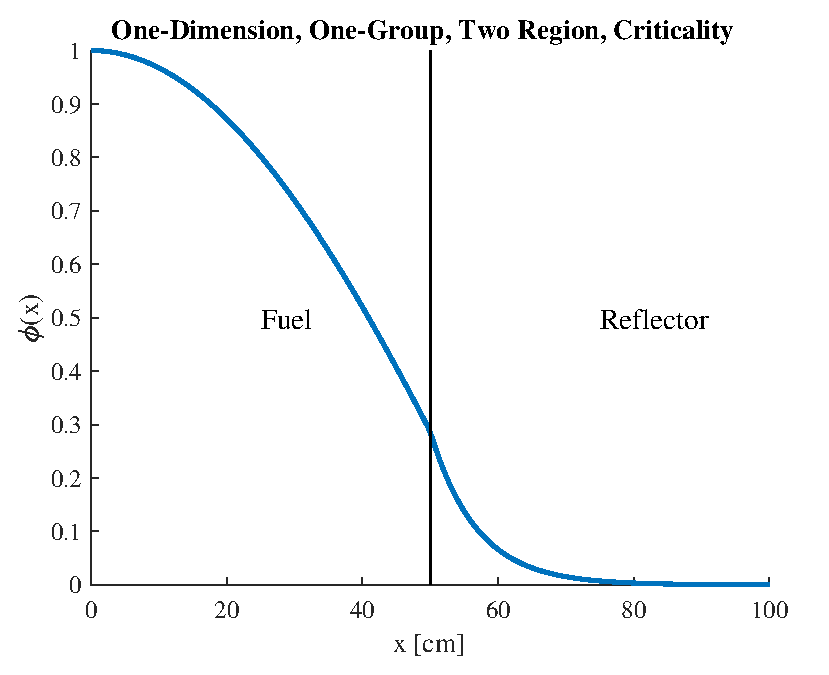
\includegraphics[width=0.7\textwidth]{2reg}
    \caption{Two Region Flux Shape.}
    \label{fig:2reg}
  \end{figure}

\section{Finite-Cylinder, One-Group, Criticality}
  \label{sec:deriv_finite_cyl}
  The finite cylinder is an example of a truly three-dimension problem with
  an analytic solution. This is a homogeneous cylinder with zero-flux boundary
  conditions on the edge of the cylinder. The cylinder has height $H$ and 
  radius $T$. The coordinates $r\in[0,T]$ and $z\in[0,H]$ where 
  $r=\sqrt{x^2+y^2}$.
  
  The solution method is by separation of variables into radial and axial 
  directions. This derivation is similar to that in \sref{sec:deriv_2d1g}.
  Beginning with the one-group neutron diffusion equation \eref{eq:onegroup} 
  and assuming that  $\phi(r,z) = R(r) Z(z)$.
  \begin{align}
    -D \grad^2 \phi(r,z) + \Sigma_r \phi(r,z) &= \nu \Sigma_f \phi(r,z) \\
    \grad^2 \phi(r,z) + \frac{\nu\Sigma_f - \Sigma_r}{D} \phi(r,g) &= 0 \\
    \frac{1}{r} \frac{\partial}{\partial r} \left( r \frac{\partial}{\partial r}
      \phi(r,z) \right) + \frac{\partial^2}{\partial z^2} \phi(r,z) +
      \frac{\nu\Sigma_f - \Sigma_r}{D} \phi(r,z) &= 0 \\
    Z(z) \frac{1}{r} \frac{\partial}{\partial r} \left( r 
      \frac{\partial}{\partial r} R(r) \right) + 
      R(r) \frac{\partial^2}{\partial z^2} Z(z) + 
      \frac{\nu\Sigma_f - \Sigma_r}{D} R(r) Z(z) &= 0 \\
    Z(z) \frac{1}{r} \frac{\partial}{\partial r} \left( r 
      \frac{\partial}{\partial r} R(r) \right) + 
      R(r) \frac{\partial^2}{\partial z^2} Z(z) + 
      B^2 R(r) Z(z) &= 0 \\
    Z(z) \left( \frac{1}{r} \frac{\partial}{\partial r} \left( r 
      \frac{\partial}{\partial r} R(r) \right) + \frac{B^2}{2} R(r) \right) + 
      R(r) \left( \frac{\partial^2}{\partial z^2} Z(z) + \frac{B^2}{2} Z(z) 
      \right) &= 0
  \end{align}
  For non-trivial solutions $R(r) \ne 0$ and $Z(z) \ne 0$ then the following
  second order ordinary differential equations can be solved.
  \begin{align}
    \label{eq:cyl_radialR}
    \frac{1}{r} \frac{\partial}{\partial r} \left( r \frac{\partial}{\partial r}
      R(r) \right) + \frac{B^2}{2} R(r) &= 0 \\
    \label{eq:cyl_axialZ}
    \frac{\partial^2}{\partial z^2} Z(z) + \frac{B^2}{2} Z(z) &= 0
  \end{align}
  
  Beginning with the axial direction. The diffusion equation can be rewritten as 
  \eref{eq:cyl_axialZ}.
  \begin{equation} \label{eq:simplediffusion}
    \grad^2 Z(z) + B_z^2 Z(z) = 0
  \end{equation}
  and has solution of the form \eref{eq:1d1g_buckle}.
  \begin{equation} \label{eq:cyl_axial}
    Z(z) = c_1 \cos(B_z z) + c_2 \sin(B_z z)
  \end{equation}
  Requiring zero-flux boundary conditions $\phi(0)=\phi(H)=0$ yields $c_1=0$. 
  Then $c_2$ is arbitrary and the buckling condition is $B_zH=\pi$ and $B_z=\pi/H$.
  
  Moving on to the radial direction. The diffusion equation can be written as
  \eref{eq:cyl_radialR}.
  \begin{equation}
    \grad^2 R(r) + B_r^2 R(r) = 0
  \end{equation}
  Noting the radial coordinates.
  \begin{align}
    \frac{1}{r} \frac{\partial}{\partial r} \left( r \frac{\partial R}
      {\partial r} \right) + B_r^2 R &= 0 \\
    \frac{\partial}{\partial r} \left( r \frac{\partial R}{\partial r}
      \right) + B_r^2 R &= 0
  \end{align}
  Noting the product rule of differentiation.
  \begin{align}
    r \frac{\partial^2 R}{\partial r^2} + \frac{\partial R}
      {\partial r} + B_r^2 r R &= 0 \\
    \frac{\partial^2 \phi}{\partial r^2} + \frac{1}{r} \frac{\partial R}
      {\partial r} + B_r^2 R &= 0 \label{eq:besselequation}
  \end{align}
  Noting equation \eref{eq:besselequation}, \cite{textbooklewis} Appendix B
  shows the equation has solution of the form
  \begin{equation} \label{eq:cyl_radial}
    R(r) = c_3 J_0(B_r r) + c_4 Y_0(B_r r)
  \end{equation}
  Where $J_0$ is the Bessel function of the first kind, zeroth order and $Y_0$
  is the Bessel function of the second kind, zeroth order. Requiring the flux
  to be finite at $r=0$ requires $c_4=0$ as 
  $\lim_{r\rightarrow0} Y_0(r) \rightarrow -\infty$. As this is an eigenvalue
  problem, $c_3$ is arbitrary. Zero flux boundary conditions requires 
  $B_r R=\alpha_0$ where $\alpha_0$ is the first root of the $J_0$ function and 
  $\alpha_0 \approx 2.4048$. Then $B_r=\alpha_0/R$.
  
  Combining the radial expression \eref{eq:cyl_radial} and the axial 
  expression \eref{eq:cyl_axial} yields the final expression for the flux.
  \begin{align} \label{eq:analytic_finite_cyl}
    \phi(r,z) &= J_0(B_r r) \sin(B_z z) \\
    &= J_0(r \alpha_0 / R) \sin(z \pi / H)
  \end{align}
  Inserting \eref{eq:analytic_finite_cyl} into the diffusion equation will yield 
  the buckling/criticality condition.
  \begin{equation}
    -D \left( \frac{1}{r} \frac{\partial}{\partial r} \left( r 
      \frac{\partial \phi}{\partial r} \right) + \frac{\partial^2 \phi}
      {\partial z^2} \right) + \Sigma_r \phi = \frac{1}{\keff} \nu 
      \Sigma_f \phi
  \end{equation}
  Beginning with the differentiation terms for simplicity. Axial 
  differentiation is straight-forward and presented below.
  \begin{equation}
    \label{eq:above}
    \frac{\partial^2 \phi}{\partial z^2} = -B_z^2 J_0(B_r r) \sin(B_z z)
  \end{equation}
  Radial differentiation must account for the radial geometry and is more 
  complex. First, note the following derivative relationship of the zeroth
  order Bessel function.
  \begin{equation} \label{eq:deriv_bessel0}
    \frac{d}{dr} J_0(\alpha r) = - \alpha J_1(\alpha r)
  \end{equation}
  And applying \eref{eq:deriv_bessel0} to \eref{eq:above}
  \begin{align}
    \frac{\partial \phi}{\partial r} &= -B_r \sin(B_z z) J_1(B_r r) \\
    r \frac{\partial \phi}{\partial r} &= -B_r \sin(B_z z) r J_1 (B_r r) 
  \end{align}
  Note the additional derivative relation for the general Bessel function.
  \begin{equation} \label{eq:deriv_besseln}
    \frac{d}{dr} J_n(r) = \frac{1}{2} \left( J_{n-1}(r) - J_{n+1}(r)\right)
  \end{equation}
  Evaluating the rest of the cylindrical derivative using
  \eref{eq:deriv_besseln} and the product rule.
  \begin{align}
    \frac{\partial}{\partial r} \left( r \frac{\partial \phi}{\partial r}
      \right) &= -B_r \sin(B_z z) \left(J_1(B_r r) + \frac{1}{2} B_r r \left(
      J_0(B_r r) - J_2(B_r r) \right) \right) \\
    \frac{1}{r} \frac{\partial}{\partial r} \left(r 
      \frac{\partial \phi}{\partial r} \right) &=
      -B_r \sin(B_z z) \left(\frac{1}{r} J_1(B_r r) + \frac{1}{2} B_r \left(
      J_0(B_r r) - J_2(B_r r) \right) \right)
  \end{align}
  Finally, inserting the expression for the Laplacian of the flux back into the
  diffusion equation.
  \begin{multline}
    D \left( B_r \sin(B_z z) \left( \frac{1}{r} J_1(B_r r) + \frac{1}{2} B_r
    \left( J_0(B_r r) - J_2(B_r r) \right) \right) + B_z^2 J_0(B_r r) \sin(B_z
    z) \right) + \Sigma_r J_0(B_r r) \sin(B_z z) = \\
    \frac{1}{\keff} \nu \Sigma_f J_0(B_r r) \sin(B_z z)
  \end{multline}
  Dividing through by $\sin(B_z z)$.
  \begin{multline}
    D \left( B_r \left( \frac{1}{r} J_1(B_r r) + \frac{1}{2} B_r
    \left( J_0(B_r r) - J_2(B_r r) \right) \right) + B_z^2 J_0(B_r r) \right)+
    \Sigma_r J_0(B_r r) = 
    \\\frac{1}{\keff} \nu \Sigma_f J_0(B_r r) 
  \end{multline}
  Dividing through by $J_0(B_r r)$ and expanding some terms.
  \begin{align}
    D \left( B_r \left( \frac{1}{r} \frac{J_1(B_r r)}{J_0(B_r r)} + 
      \frac{1}{2} \left(B_r - \frac{J_2(B_r r)}{J_0(B_r r)} \right) \right) 
      + B_z^2 \right)+ \Sigma_r &= \frac{1}{\keff} \nu \Sigma_f \\
    D \left( \frac{1}{r} B_r \frac{J_1(B_r r)}{J_0(B_r r)} + \frac{B_r^2}{2} -
      \frac{B_r^2}{2} \frac{J_2(B_r r)}{J_0(B_r r)} + B_z^2 \right) + \Sigma_r&=
      \frac{1}{\keff} \nu \Sigma_f  \\
    \frac{1}{r} B_r \frac{J_1(B_r r)}{J_0(B_r r)} + \frac{B_r^2}{2} -
      \frac{B_r^2}{2} \frac{J_2(B_r r)}{J_0(B_r r)} + B_z^2 + 
      \frac{\Sigma_r}{D} &= \frac{1}{\keff} \frac{\nu \Sigma_f}{D}\\
    \frac{1}{J_0(B_r r)} \frac{B_r^2}{2} \left(\frac{1}{r} \frac{2}{B_r} 
      J_1(B_r r) - J_2(B_r r) \right) + \frac{B_r^2}{2} + B_z^2 + 
      \frac{\Sigma_r}{D} &= \frac{1}{\keff} \frac{\nu \Sigma_f}{D}
  \end{align}
  Note the Bessel function recursion relationship.
  \begin{equation} \label{eq:bessel_recursion}
    J_{n+1}(\alpha r) + J_{n-1}(\alpha r) = \frac{2n}{\alpha r} J_n(\alpha r)
  \end{equation}
  Using \eref{eq:bessel_recursion} the term above is simplified.
  \begin{align}
    \frac{1}{J_0(B_r r)} \frac{B_r^2}{2} \left( J_0(B_r r) \right) + 
      \frac{B_r^2}{2} + B_z^2 + \Sigma_r &= \frac{1}{\keff} 
      \frac{\nu \Sigma_f}{D} \\
    B_r^2 + B_z^2 + \frac{\Sigma_r}{D} &= \frac{1}{\keff} \frac{\nu \Sigma_f}
      {D}
  \end{align}
  Now, an expression for the eigenvalue can be written.
  \begin{align}
    \keff &= \frac{\nu \Sigma_f}{D(B_r^2 + B_z^2) + \Sigma_r} \\
    &= \frac{\nu \Sigma_f}{D\left(\left(\frac{\alpha_0}{R}\right)^2 + 
      \left(\frac{\pi}{H}\right)^2 \right) + \Sigma_r} \\
    &= 0.996710620898177
  \end{align}
  NOTE: the shape of the boundary is extremely important for this  problem.
  Therefore, the mesh must be regenerated with a halved mesh parameter  $h$ for
  each refinement, rather than simply splitting nodes as splitting nodes would 
  not improve the description of the boundary.

